\documentclass[aspectratio=169]{beamer}
\usetheme{Madrid}
\usecolortheme{whale}

\usepackage[utf8]{vietnam}
\usepackage{graphicx}
\usepackage{tikz}
\usetikzlibrary{arrows.meta,positioning}

\title{Lý thuyết đồ thị}
\author{Nhóm 7}
\date{\today}

\begin{document}

%------------------------------------------------
\begin{frame}
\titlepage
\end{frame}

%------------------------------------------------
\begin{frame}{Nội dung}
\tableofcontents
\end{frame}

%================================================
\section{Định nghĩa đồ thị}

%------------------------------------------------
\begin{frame}{Đồ thị là gì}

\begin{itemize}

\item Đồ thị là cấu trúc dữ liệu mô tả mối quan hệ giữa các đối tượng.

\item Ký hiệu:

\[
G = (V,E)
\]

\item $V$ là tập các đỉnh

\item $E$ là tập các cạnh

\item Mỗi cạnh nối hai đỉnh của đồ thị

\end{itemize}

\end{frame}

%------------------------------------------------
\begin{frame}{Ví dụ đồ thị}

\begin{center}

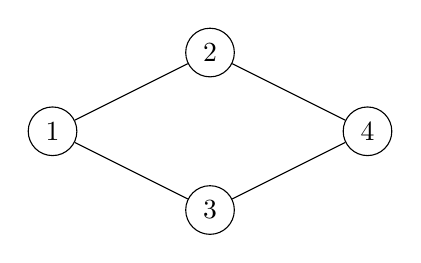
\begin{tikzpicture}

\node[circle,draw] (1) at (0,0) {1};
\node[circle,draw] (2) at (2,1) {2};
\node[circle,draw] (3) at (2,-1) {3};
\node[circle,draw] (4) at (4,0) {4};

\draw (1)--(2);
\draw (1)--(3);
\draw (2)--(4);
\draw (3)--(4);

\end{tikzpicture}

\end{center}

\end{frame}

%------------------------------------------------

\begin{frame}{Phân loại đồ thị}

\begin{itemize}
    \item $G$ được gọi là \textbf{đơn đồ thị} nếu giữa hai đỉnh $u, v$ của $V$ có nhiều nhất là $1$ cạnh trong $E$ nối từ $u$ tới $v$.
    
    \item $G$ được gọi là \textbf{đa đồ thị} nếu giữa hai đỉnh $u, v$ của $V$ có thể có nhiều hơn $1$ cạnh trong $E$ nối từ $u$ tới $v$ (Hiển nhiên đơn đồ thị cũng là đa đồ thị).
    
    \item $G$ được gọi là \textbf{đồ thị vô hướng} nếu các cạnh trong $E$ là không định hướng, tức là cạnh nối hai đỉnh $u, v$ bất kỳ cũng là cạnh nối hai đỉnh $v, u$. Hay nói cách khác, tập $E$ gồm các cặp $(u, v)$ không tính thứ tự: $(u, v) \equiv (v, u)$.
    
    \item $G$ được gọi là \textbf{đồ thị có hướng} nếu các cạnh trong $E$ là có định hướng, có thể có cạnh nối từ đỉnh $u$ tới đỉnh $v$ nhưng chưa chắc đã có cạnh nối từ đỉnh $v$ tới đỉnh $u$. Hay nói cách khác, tập $E$ gồm các cặp $(u, v)$ có tính thứ tự: $(u, v) \neq (v, u)$. Trong đồ thị có hướng, các cạnh được gọi là các \textbf{cung}. Đồ thị vô hướng cũng có thể coi là đồ thị có hướng nếu như ta coi cạnh nối hai đỉnh $u, v$ bất kỳ tương đương với hai cung $(u, v)$ và $(v, u)$.
\end{itemize}

\end{frame}

%-----------------------------------------------
\begin{frame}{Phân loại đồ thị}

\begin{center}

\includegraphics[width=1\textwidth]{Don_da_do_thi.png}

\end{center}

\end{frame}
%================================================
\section{Ứng dụng của đồ thị}

\begin{frame}{Ứng dụng của đồ thị}
\begin{itemize}
  \item Mạng xã hội: Mỗi người là một đỉnh, mỗi mối quan hệ là một cạnh.
  \item Mạng máy tính: Mỗi máy tính là một đỉnh, mỗi kết nối là một cạnh.
  \item Định tuyến: Tìm đường đi ngắn nhất giữa hai điểm.
  \item Lập lịch: Mỗi công việc là một đỉnh, mỗi phụ thuộc là một cạnh.
  \item Sinh học: Mô hình hóa mối quan hệ giữa các gen hoặc protein.
\end{itemize}
\end{frame}
%------------------------------------------------

%================================================
\section{Biểu diễn đồ thị}

%------------------------------------------------
\begin{frame}{Ma trận kề}

\begin{itemize}

\item Sử dụng mảng hai chiều $A[n][n]$

\item Nếu tồn tại cạnh $(u,v)$ thì

\[
A[u][v] = 1
\]

\item Nếu không tồn tại cạnh thì

\[
A[u][v] = 0
\]

\end{itemize}

\begin{block}{Độ phức tạp}

\begin{itemize}

\item Kiểm tra cạnh $(u,v)$: $O(1)$

\item Duyệt các đỉnh kề: $O(V)$

\item Bộ nhớ sử dụng: $O(V^2)$

\end{itemize}

\end{block}

\end{frame}

%------------------------------------------------
\begin{frame}{Danh sách kề}

\begin{itemize}

\item Mỗi đỉnh lưu danh sách các đỉnh kề

\item Cấu trúc thường dùng:

\begin{center}

vector<int> adj[N]

\end{center}

\item Ví dụ:

\begin{itemize}

\item adj[1] = {2,3}

\item adj[2] = {4}

\end{itemize}

\end{itemize}

\begin{block}{Độ phức tạp}

\begin{itemize}

\item Kiểm tra cạnh $(u,v)$: $O(deg(u))$

\item Duyệt các đỉnh kề: $O(deg(u))$

\item Bộ nhớ sử dụng: $O(V+E)$

\end{itemize}

\end{block}

\end{frame}
%================================================
\section{Một số thuật toán duyệt đồ thị}

%------------------------------------------------
\begin{frame}{Thuật toán DFS}

\begin{itemize}

\item DFS (Depth First Search)

\item Đi sâu nhất có thể trước khi quay lui

\item Dùng đệ quy hoặc stack

\end{itemize}

\begin{block}{Độ phức tạp}

\[
O(V+E)
\]

\end{block}

\end{frame}

%------------------------------------------------
\begin{frame}[fragile]{Code DFS}

\begin{verbatim}
void dfs(int u)
{
 visited[u]=true;

 for(int v:adj[u])
 {
  if(!visited[v])
   dfs(v);
 }
}
\end{verbatim}

\end{frame}

%------------------------------------------------
\begin{frame}{Mô phỏng DFS}

\begin{center}

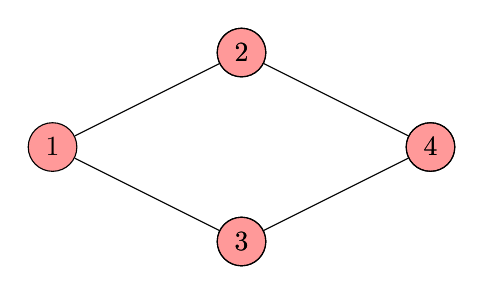
\begin{tikzpicture}[scale=1.2]

\node[circle,draw,fill=red!40] (1) at (0,0) {1};

\node<2->[circle,draw,fill=red!40] (2) at (2,1) {2};
\node[circle,draw] (2a) at (2,1) {2};

\node<3->[circle,draw,fill=red!40] (4) at (4,0) {4};
\node[circle,draw] (4a) at (4,0) {4};

\node<4->[circle,draw,fill=red!40] (3) at (2,-1) {3};
\node[circle,draw] (3a) at (2,-1) {3};

\draw (1)--(2a);
\draw (1)--(3a);
\draw (2a)--(4a);
\draw (3a)--(4a);

\end{tikzpicture}

\end{center}

\begin{itemize}

\item<1-> Bắt đầu từ đỉnh 1
\item<2-> Đi tới đỉnh 2
\item<3-> Đi tiếp tới đỉnh 4
\item<4-> Quay lui và thăm đỉnh 3

\end{itemize}

\end{frame}

%------------------------------------------------
\begin{frame}{Thuật toán BFS}

\begin{itemize}

\item BFS (Breadth First Search)

\item Duyệt theo từng lớp

\item Sử dụng Queue

\end{itemize}

\end{frame}

%------------------------------------------------
\begin{frame}[fragile]{Code BFS}

\begin{verbatim}

queue<int> q;

q.push(s);
visited[s]=true;

while(!q.empty())
{
 int u=q.front();
 q.pop();

 for(int v:adj[u])
  if(!visited[v])
  {
   visited[v]=true;
   q.push(v);
  }
}

\end{verbatim}

\end{frame}

%------------------------------------------------
\begin{frame}{Mô phỏng BFS}

\begin{center}

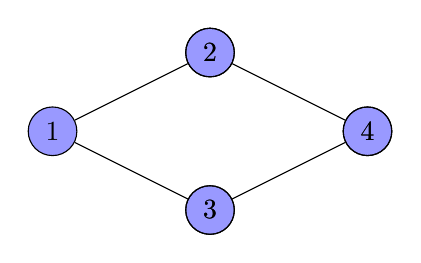
\begin{tikzpicture}

\node<1->[circle,draw,fill=blue!40] (1) at (0,0) {1};

\node<2->[circle,draw,fill=blue!40] (2) at (2,1) {2};
\node[circle,draw] (2a) at (2,1) {2};

\node<2->[circle,draw,fill=blue!40] (3) at (2,-1) {3};
\node[circle,draw] (3a) at (2,-1) {3};

\node<3->[circle,draw,fill=blue!40] (4) at (4,0) {4};
\node[circle,draw] (4a) at (4,0) {4};

\draw (1)--(2a);
\draw (1)--(3a);
\draw (2a)--(4a);
\draw (3a)--(4a);

\end{tikzpicture}

\end{center}

\begin{itemize}

\item<1-> Bắt đầu tại đỉnh 1
\item<2-> Thăm các đỉnh cùng lớp: 2 và 3
\item<3-> Sau đó đến đỉnh 4

\end{itemize}

\end{frame}

%================================================

\section{Kết luận}

%------------------------------------------------
\begin{frame}{Tổng kết}

\begin{itemize}

\item Đồ thị là cấu trúc dữ liệu quan trọng

\item DFS và BFS dùng để duyệt đồ thị

\item Dijkstra tìm đường đi ngắn nhất

\item Có nhiều ứng dụng trong thực tế

\end{itemize}

\end{frame}

%------------------------------------------------
\begin{frame}

\centering
\Huge
Cảm ơn các bạn đã lắng nghe!

\end{frame}

\end{document}